\documentclass[12pt]{beamer}

\usetheme[progressbar=frametitle]{metropolis}
\usepackage{appendixnumberbeamer}

\usepackage[autoplay]{animate}
\usepackage{graphicx}
\usepackage{subcaption}
\usepackage{coloremoji}

\usepackage{booktabs}
\usepackage[scale=2]{ccicons}

%\usepackage{pgfplots}
%\usepgfplotslibrary{dateplot}

\usepackage{xspace}

\newcommand\blfootnote[1]{%
  \begingroup
  \renewcommand\thefootnote{}\footnote{#1}%
  \addtocounter{footnote}{-1}%
  \endgroup
}

\setbeamercolor{normal text}{bg=white}
\newcommand{\themename}{\textbf{\textsc{metropolis}}\xspace}

\title{Introduktion till Docker}
\subtitle{Och kontainrar i allmänhet}
\date{\today}
\author{Simon Rydell}

% \titlegraphic{\hfill\includegraphics[height=1.5cm]{logo.pdf}}

\begin{document}

\begin{frame}
\titlepage
\end{frame}

%    \begin{columns}[c]
%        \column{4in}
%            \begin{figure}[h!]
%                \centering
%                \includegraphics[width=.8\textwidth]{../figures/learingCurve.pdf}
%            \end{figure}
%    \end{columns}

%\maketitle
% 
\begin{frame}{Kontainer?}
    \begin{columns}
        \column{.25in}
        \column{2in}
        \begin{itemize}
            \item "Kappsla in'' processer
            \item Garanterar samma miljö för ett program
        \end{itemize}
        \column{2.5in}
            \begin{figure}[h!]
                \centering
                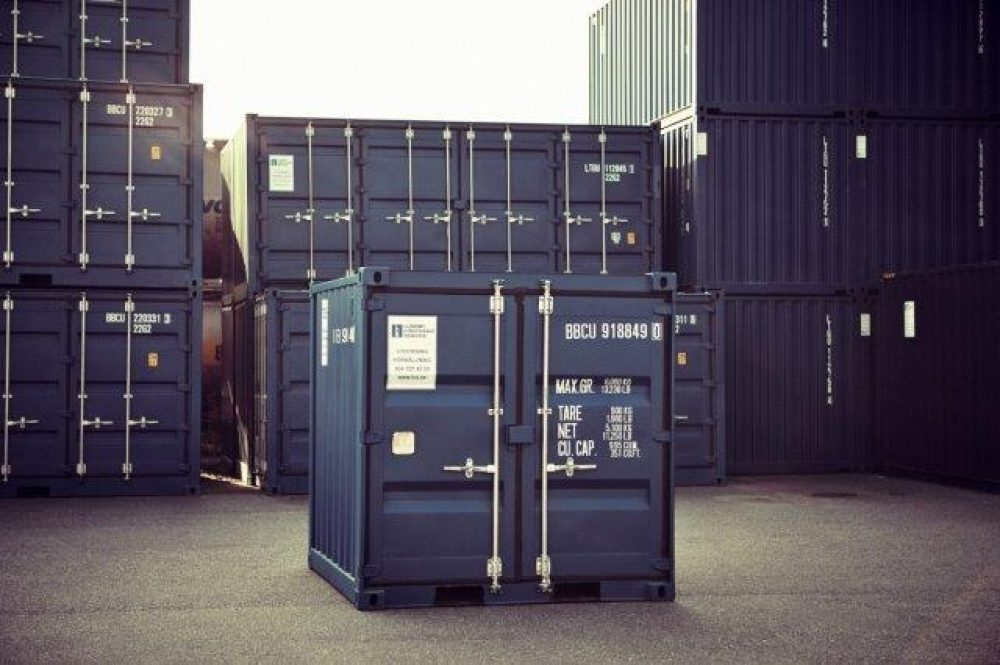
\includegraphics[width=.8\textwidth]{../figures/one_container.jpg}
            \end{figure}
    \end{columns}
     \blfootnote{github.com/srydell/docker-intro}
\end{frame}

% 
\begin{frame}{Översikt}
    \setbeamertemplate{section in toc}[sections numbered]
    \tableofcontents[hideallsubsections]
    \blfootnote{github.com/srydell/docker-intro}
\end{frame}

% --- Section ---
\section{Virtual machine vs container}

\begin{frame}{Virtual Machine (VM)}
    \begin{columns}
        \column{.25in}
        \column{2in}
        \begin{itemize}
            \item Virtualisera allt! (Nästan)
            \item Tunga processer
            \item Som en dator
        \end{itemize}
        \column{2.5in}
            \begin{figure}[h!]
                \centering
                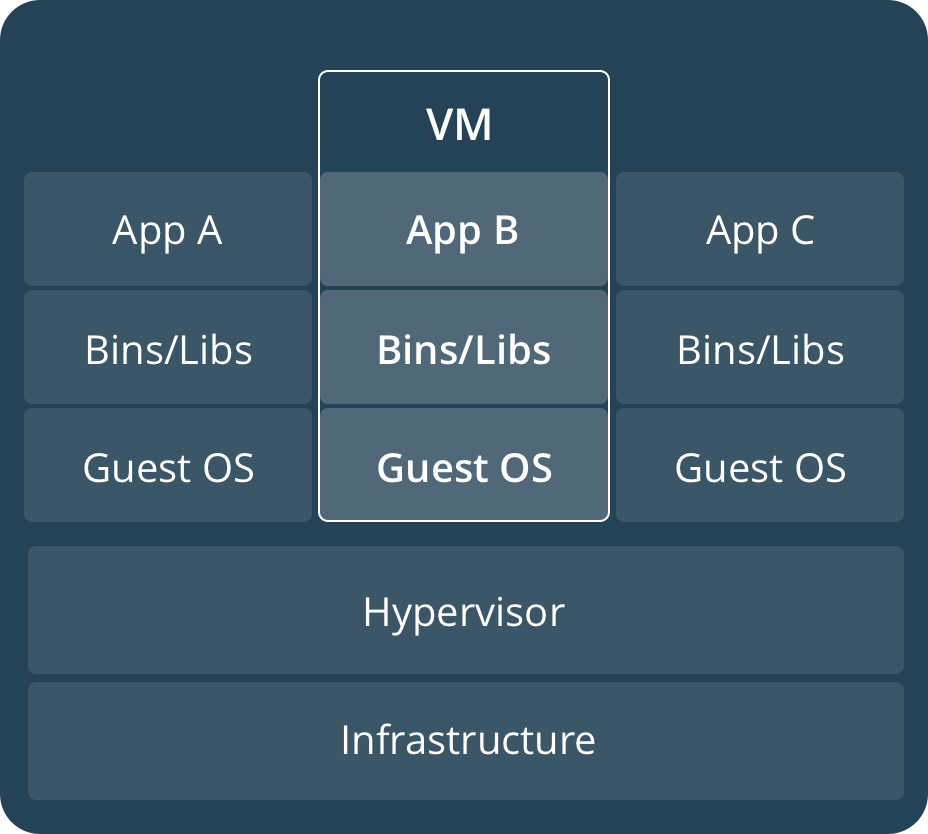
\includegraphics[width=.8\textwidth]{../figures/vm.png}
            \end{figure}
    \end{columns}
    \blfootnote{github.com/srydell/docker-intro}
\end{frame}

\begin{frame}{Container - Docker}
    \begin{columns}
        \column{2.5in}
            \begin{figure}[h!]
                \centering
                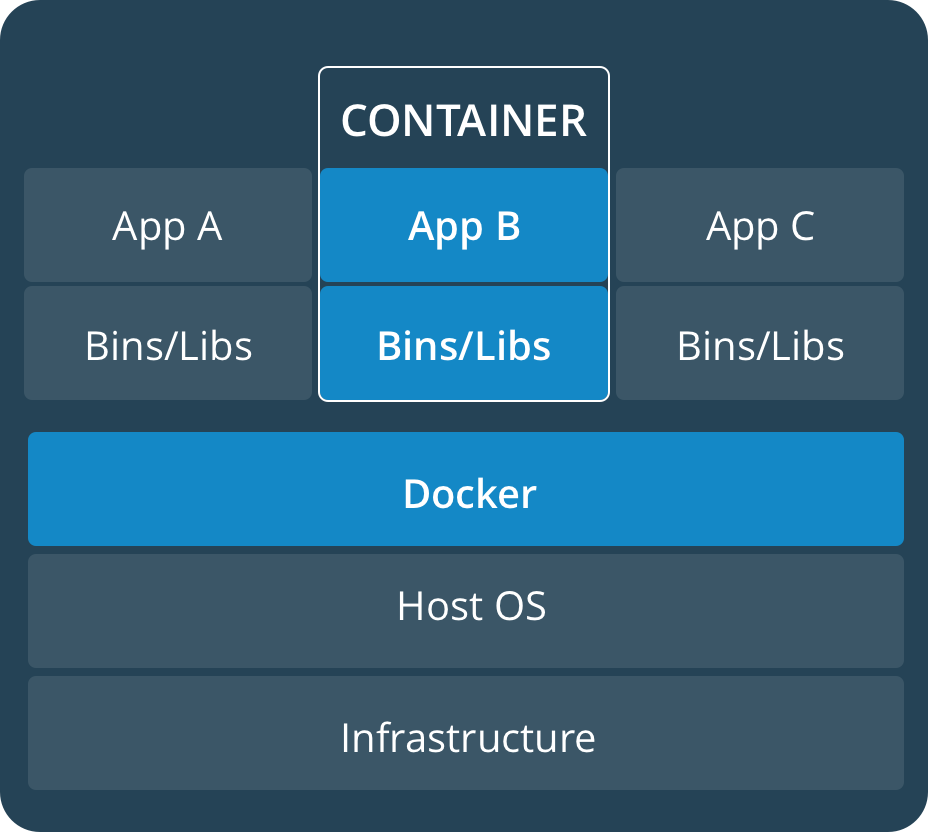
\includegraphics[width=.8\textwidth]{../figures/containers.png}
            \end{figure}
        \column{2.5in}
            \begin{itemize}
                \item Virtualisera det som behövs
                \item "Lättviktiga" processer
                \item Som en samling processer
            \end{itemize}
        \end{columns}
    \blfootnote{github.com/srydell/docker-intro}
\end{frame}

\begin{frame}{Virtual machine vs container}
    \begin{columns}
        \column{2.5in}
            \begin{figure}[h!]
                \centering
                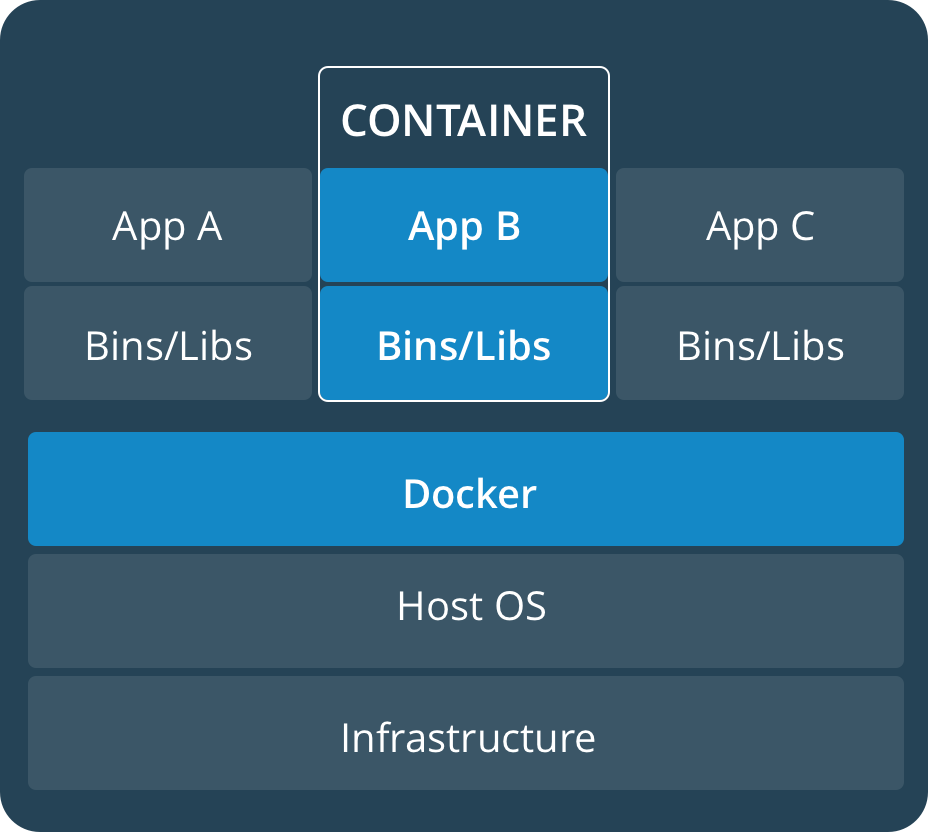
\includegraphics[width=.8\textwidth]{../figures/containers.png}
            \end{figure}
        \column{2.5in}
            \begin{figure}[h!]
                \centering
                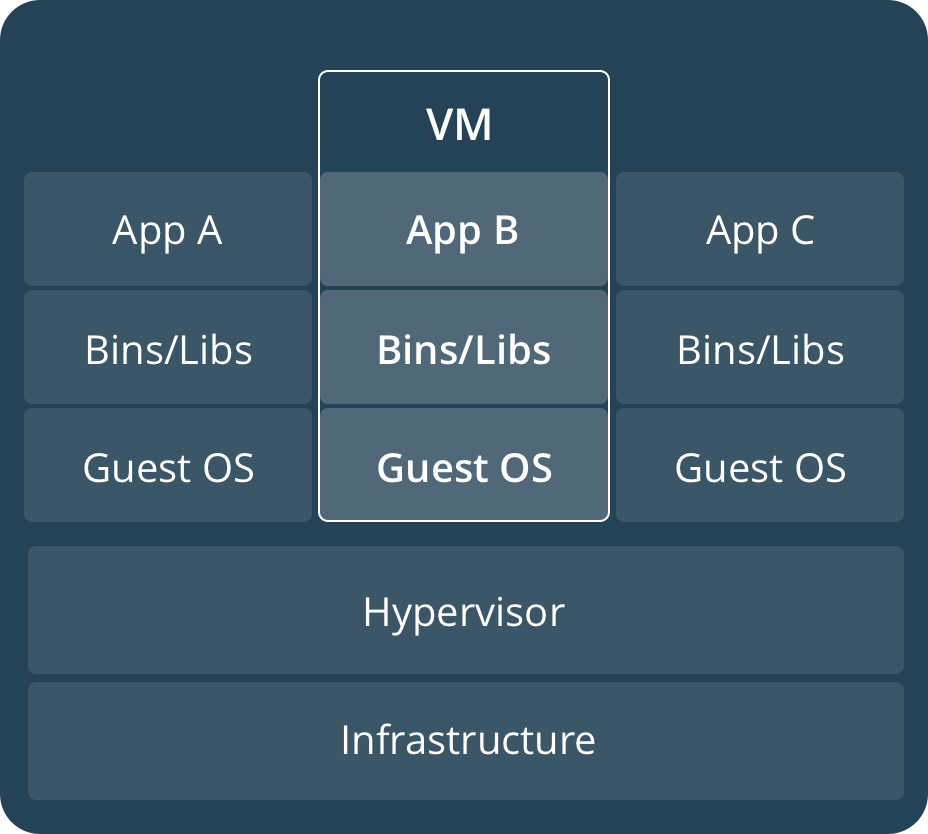
\includegraphics[width=.8\textwidth]{../figures/vm.png}
            \end{figure}
    \end{columns}
    \blfootnote{github.com/srydell/docker-intro}
\end{frame}

% --- Section ---
\section{Använda Docker}

\begin{frame}{Dockerfile}
   \begin{columns}
        \column{.25in}
        \column{2in}
        \begin{itemize}
            \item Som okompilerad kod - måste byggas för att köras
            \item Om du kan göra det via terminal kan du göra det genom Docker
        \end{itemize}
        \column{2.5in}
            \begin{figure}[h!]
                \centering
                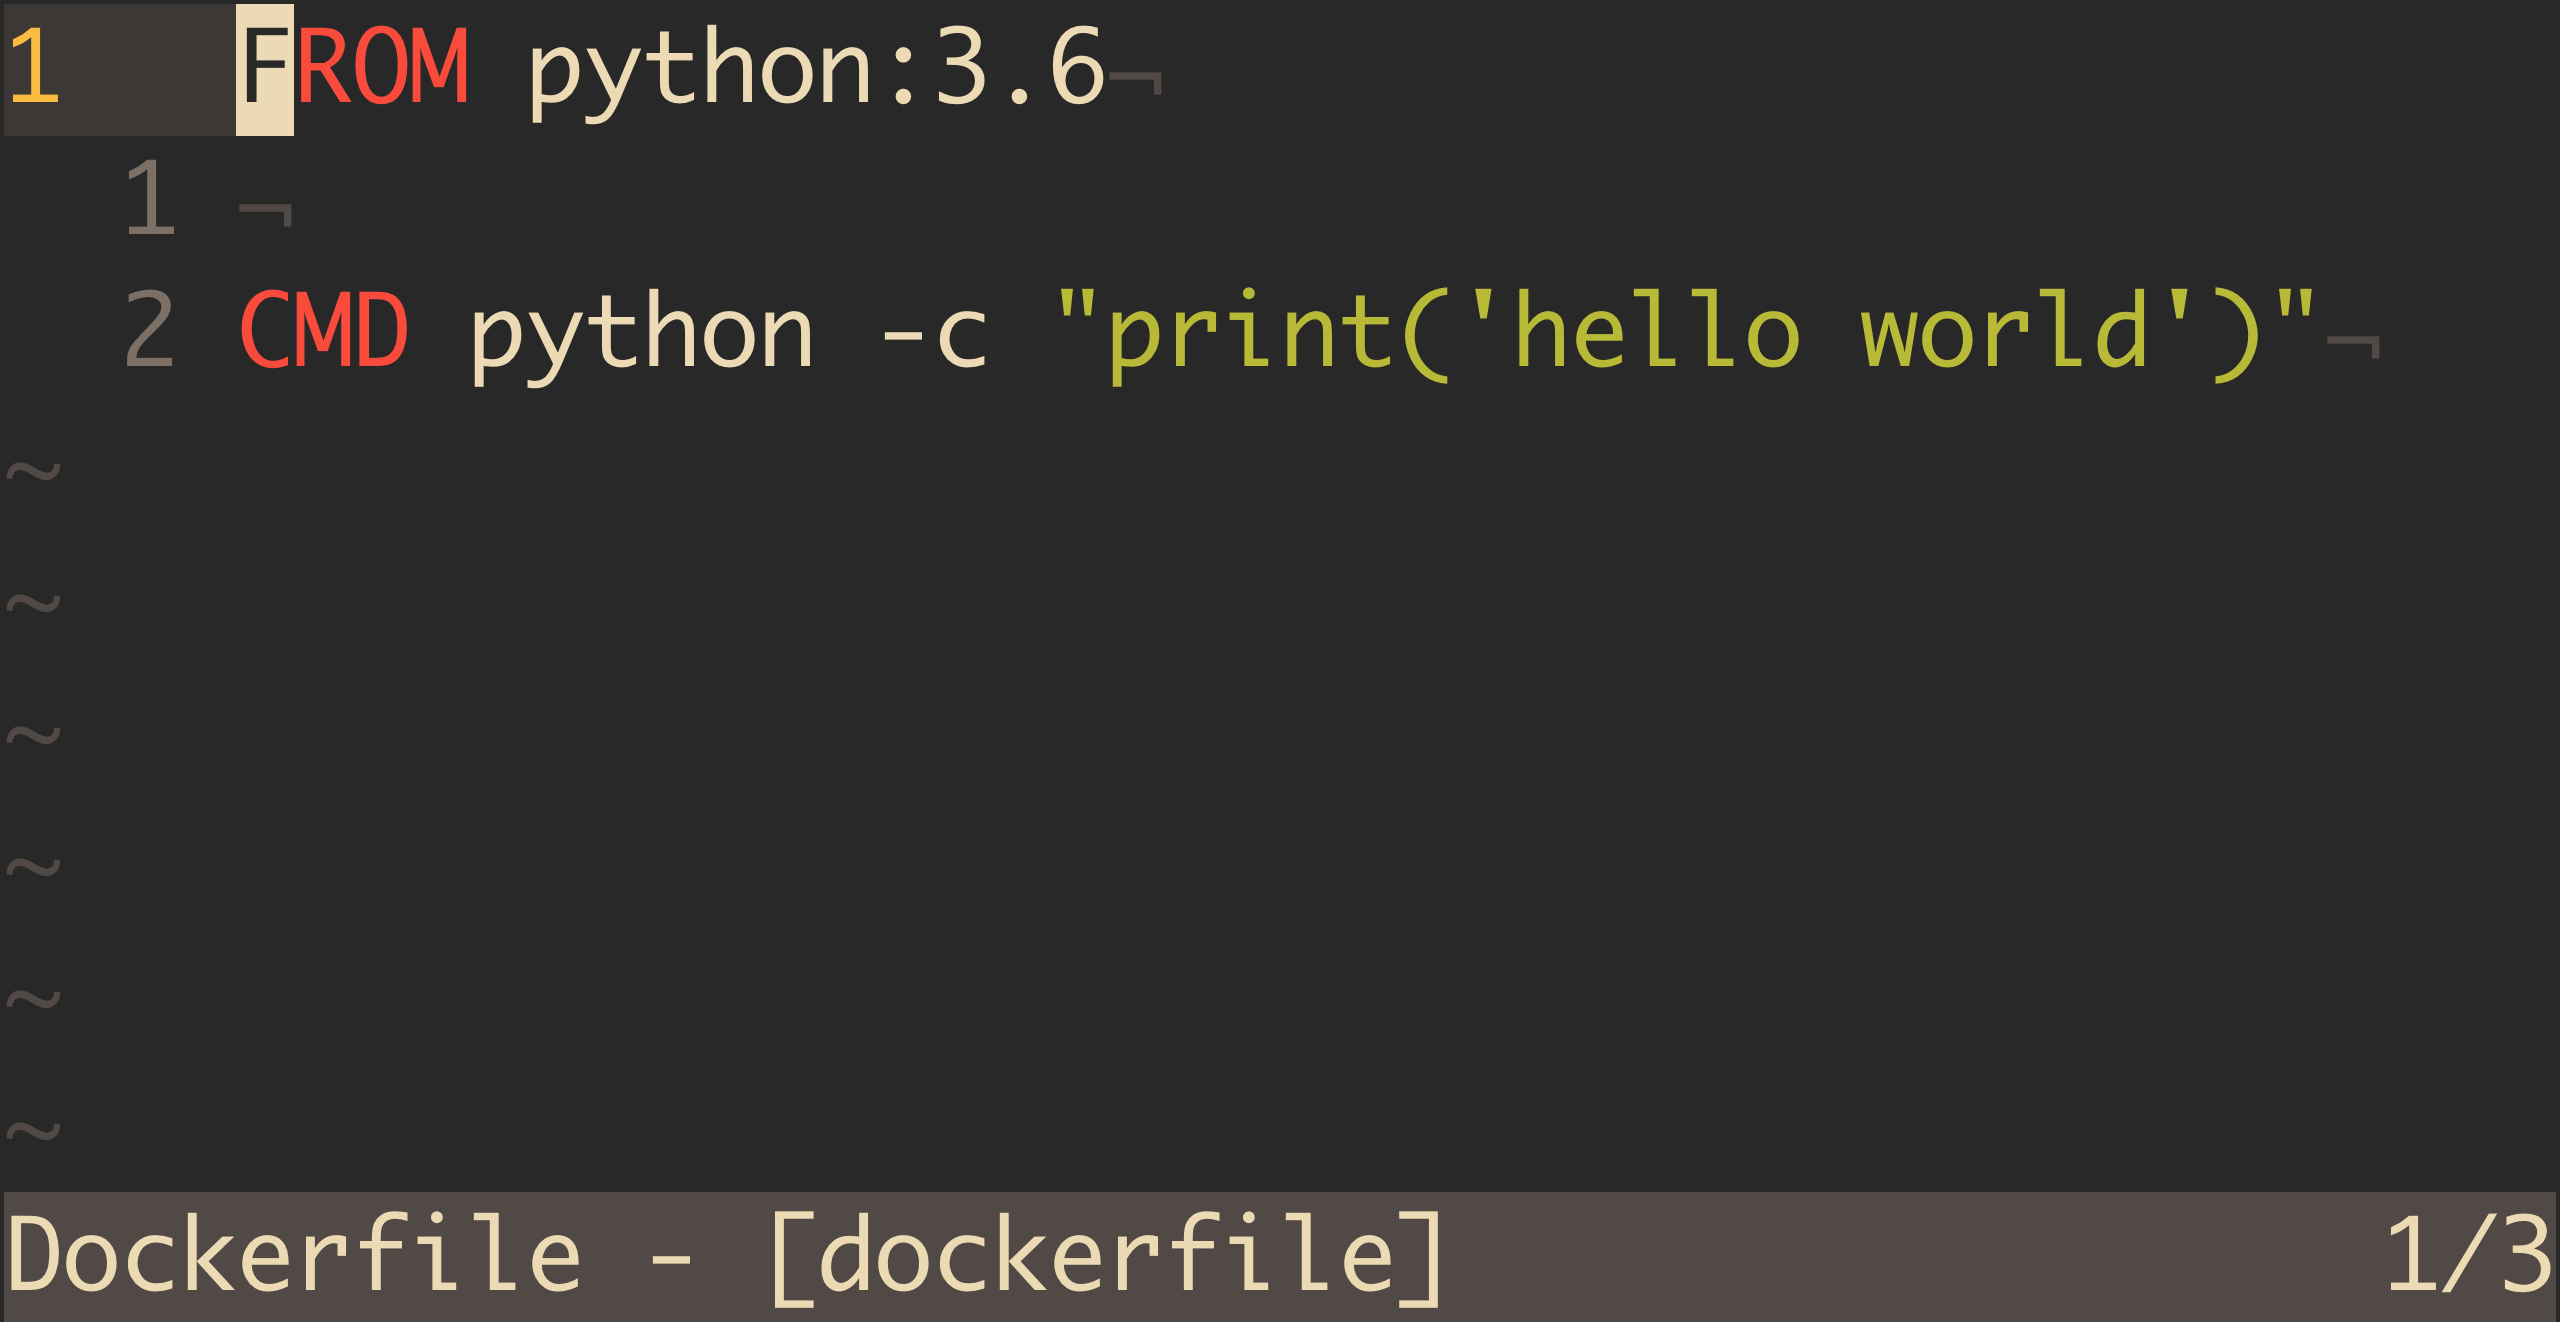
\includegraphics[width=.8\textwidth]{../figures/simpleDockerfile.png}
            \end{figure}
    \end{columns}
    \blfootnote{github.com/srydell/docker-intro}
\end{frame}

\begin{frame}{Docker registry - Dockerhub}
    \begin{itemize}
        \item Som ett git server där varje repository är Dockerfiles \\(eller images)
        \item Används oftast direkt från $FROM$ i en Dockerfile
    \end{itemize}
    \blfootnote{github.com/srydell/docker-intro}
\end{frame}
% --- Section ---
\section{Exempel}

\begin{frame}{Exempel}
     \begin{itemize}
         \item Bygga en Dockerfile
         \begin{itemize}
             \item Command line intro
         \end{itemize}
         \item Jenkins
         \begin{itemize}
             \item Exponera portar
             \item Daemons
             \item Volumes
         \end{itemize}
     \end{itemize}
     \blfootnote{github.com/srydell/docker-intro}
\end{frame}

\begin{frame}{Vad jag inte tog upp}
    \begin{itemize}
        \item Network - Hur kontainrar ser varandras nätverk
        \item Logging - Hur samlar man fel/loggar på ett effektivt sätt
        \item Orchestration - Hur man kopplar ihop kontainrar
    \end{itemize}
     \blfootnote{github.com/srydell/docker-intro}
\end{frame}

\begin{frame}{Docker introduktion}
    \begin{center}
    \LARGE Frågor
    \end{center}
    \blfootnote{github.com/srydell/docker-intro}
\end{frame}


\end{document}